\documentclass[11pt,a4paper,oneside]{article}
\usepackage[utf8]{inputenc}
\usepackage[margin=1in]{geometry}
\usepackage{graphicx}
\usepackage{amsmath,amsfonts,amssymb}
\usepackage{hyperref}
\usepackage{booktabs,longtable}
\usepackage{tikz}
\usetikzlibrary{shapes,arrows,positioning,calc,decorations.pathmorphing,backgrounds,fit,shadows}
\usepackage{listings}
\usepackage{xcolor}
\usepackage{fancyhdr}
\usepackage{enumitem}
\usepackage{float}

\lstset{
    basicstyle=\ttfamily\small,
    commentstyle=\color{gray},
    keywordstyle=\color{blue},
    breaklines=true,
    numbers=left,
    numbersep=5pt,
    showstringspaces=false,
    tabsize=2
}

\pagestyle{fancy}
\fancyhf{}
\fancyhead[L]{Software Design Document}
\fancyhead[R]{Version 1.0}
\fancyfoot[C]{\thepage}

\hypersetup{
    colorlinks=true,
    linkcolor=blue,
    urlcolor=cyan,
    pdftitle={Unknown.  Could be a web application, mobile application, API, or another type of software.  More information is needed. Design Document},
    pdfauthor={AI Generated},
    pdfsubject={Software Architecture}
}

\title{\textbf{Unknown.  Could be a web application, mobile application, API, or another type of software.  More information is needed. - Software Design Document}}
\author{AI System Architect}
\date{\today}

\begin{document}

\maketitle
\thispagestyle{empty}
\newpage

\tableofcontents
\newpage

\section{Executive Summary}

This software design document outlines the architecture and implementation strategy for a unknown.  could be a web application, mobile application, api, or another type of software.  more information is needed.. Based on the analyzed requirements, this system will implement unknown.  a monolithic architecture would be simplest for a small project, while microservices might be better for larger, more complex projects.  the choice depends on anticipated scale and complexity, which are unknown. architecture with a focus on unable to determine.  no features are described in the provided extract.  examples would include: user authentication and data input.

\subsection{Project Overview}

The system is designed to address the following key requirements:
\item Unable to determine. No features are described in the provided extract. Examples would include: User authentication
\item data input
\item data processing
\item reporting
\item etc. These are placeholders and need to be replaced with actual requirements.

\subsection{Technology Stack}

The recommended technology stack includes:
\item Unable to determine. This depends heavily on the project type and features. A possible (but generic) example:
\item Frontend: React (if web app)
\item React Native (if mobile app)
\item Backend: Node.js with Express.js (or similar framework like Python/Django
\item Java/Spring Boot)
\item Database: PostgreSQL or MySQL

\section{Requirements Analysis}

\subsection{Extracted Requirements Summary}

Based on the document analysis, the following content was identified:

\begin{quote}
No content extracted
\end{quote}

\subsection{Functional Requirements}

The system shall provide the following key functionalities:
\begin{enumerate}
\item Unable to determine. No features are described in the provided extract. Examples would include: User authentication
\item data input
\item data processing
\item reporting
\item etc. These are placeholders and need to be replaced with actual requirements.
\end{enumerate}

\subsection{Non-Functional Requirements}

Based on the analysis, the system must meet these requirements:
\begin{itemize}
\item \textbf{Performance}: Optimized for unknown.  could be a web application, mobile application, api, or another type of software.  more information is needed. workloads
\item \textbf{Scalability}: Scalable architecture supporting growth
\item \textbf{Security}: Unable to determine. General security considerations include:, Authentication and Authorization: Secure user login and access control., Data Protection: Encryption of sensitive data at rest and in transit., Input Validation: Sanitize user inputs to prevent injection attacks., Regular Security Audits: To identify and address vulnerabilities.
\item \textbf{Availability}: High availability deployment strategy
\end{itemize}

\section{System Architecture}

\subsection{Architecture Overview}

The system follows a unknown.  a monolithic architecture would be simplest for a small project, while microservices might be better for larger, more complex projects.  the choice depends on anticipated scale and complexity, which are unknown. pattern optimized for unknown.  could be a web application, mobile application, api, or another type of software.  more information is needed. development.


\begin{figure}[H]
\centering
\begin{tikzpicture}[
    node distance=1cm and 1.5cm,
    font=\sffamily\small,
    base/.style={draw, text width=3cm, minimum height=1.2cm, text centered, rounded corners, drop shadow},
    user/.style={base, fill=Azure!30, text width=2cm},
    api/.style={base, fill=LimeGreen!20},
    service/.style={base, fill=SkyBlue!20},
    database/.style={cylinder, shape border rotate=90, aspect=0.25, draw, fill=Thistle!40, minimum height=1.5cm, text width=2.5cm, text centered, drop shadow},
    external/.style={base, fill=Gold!30},
    arrow/.style={-Stealth, thick, draw=black!60}
]

\node[user] (user) {User};
\node[api, below=1.5cm of user] (gateway) {API Gateway};
\node[service, below=of gateway, xshift=-3cm] (auth) {Authentication Service};
\node[service, below=of gateway] (business) {Business Logic Service};
\node[service, below=of gateway, xshift=3cm] (data) {Data Processing Service};
\node[database, below=2cm of auth] (authdb) {User Database\\(PostgreSQL)};
\node[database, below=2cm of business] (maindb) {Application DB\\(MongoDB)};
\node[database, below=2cm of data] (cache) {Cache and Queues\\(Redis/RabbitMQ)};
\node[external, right=2cm of business] (payment) {External Services\\(Payment, Email)};

\begin{scope}[on background layer]
\node[draw, dashed, rounded corners, fill=gray!5, inner sep=0.7cm, fit=(gateway)] (api_layer) {};
\node[draw, dashed, rounded corners, fill=gray!10, inner sep=0.7cm, fit=(auth) (business) (data) (payment)] (service_layer) {};
\node[draw, dashed, rounded corners, fill=gray!15, inner sep=0.7cm, fit=(authdb) (maindb) (cache)] (data_layer) {};
\end{scope}

\node[above] at (api_layer.north) {API Layer};
\node[above] at (service_layer.north) {Service Layer};
\node[above] at (data_layer.north) {Data Layer};

\draw[arrow] (user) -- (gateway);
\draw[arrow] (gateway) -- (auth);
\draw[arrow] (gateway) -- (business);
\draw[arrow] (gateway) -- (data);
\draw[arrow] (auth) -- (authdb);
\draw[arrow] (business) -- (maindb);
\draw[arrow] (business) -- (payment);
\draw[arrow] (data) -- (cache);
\draw[arrow] (business) -- (data);

\end{tikzpicture}
\caption{Modern System Architecture Overview}
\label{fig:architecture}
\end{figure}


\subsection{Architecture Rationale}

The Unknown.  A monolithic architecture would be simplest for a small project, while microservices might be better for larger, more complex projects.  The choice depends on anticipated scale and complexity, which are unknown. architecture was chosen because:
\begin{itemize}
\item Optimal for unknown. could be a web application, mobile application, api, or another type of software. more information is needed. requirements
\item Supports scalable unknown. a monolithic architecture would be simplest for a small project, while microservices might be better for larger, more complex projects. the choice depends on anticipated scale and complexity, which are unknown. design
\item Enables independent development and deployment
\item Provides fault tolerance and resilience
\end{itemize}

\section{Database Design}

\subsection{Data Model}

Based on the requirements analysis, the following key entities were identified:
\begin{itemize}
\item \textbf{Unable to determine. Examples (placeholders): Users}: Core data entity
\item \textbf{Products}: Core data entity
\item \textbf{Orders}: Core data entity
\item \textbf{Transactions. These are purely speculative and must be replaced with actual entities based on the application's requirements.}: Core data entity
\end{itemize}


\begin{figure}[H]
\centering
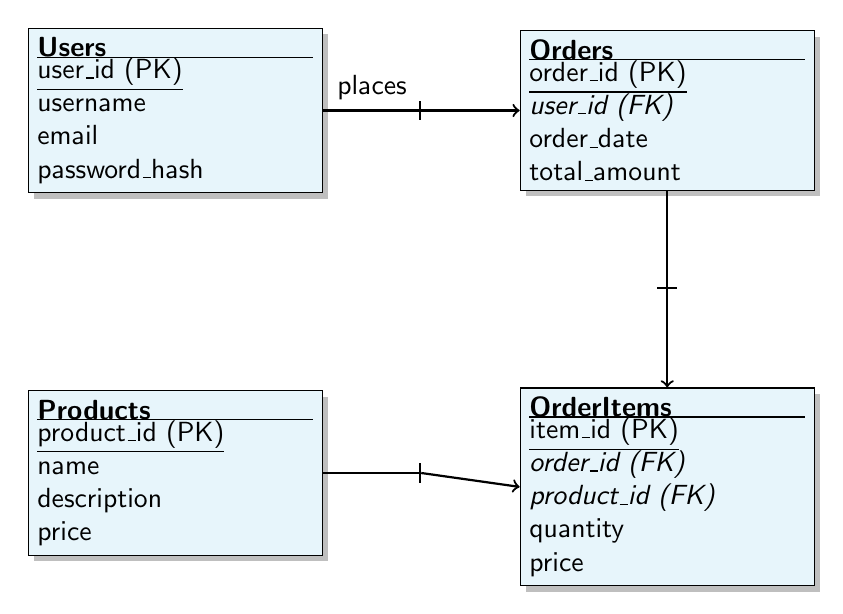
\begin{tikzpicture}[
    node distance=2.5cm,
    font=\sffamily,
    entity/.style={rectangle, draw, fill=SkyBlue!20, text width=3.5cm, minimum height=2cm, align=left, drop shadow},
    one/.style={-|, thick},
    many/.style={->, thick}
]

\node[entity] (user) {\textbf{Users} \\ \hrule \underline{user\_id (PK)} \\ username \\ email \\ password\_hash};
\node[entity, right=of user] (order) {\textbf{Orders} \\ \hrule \underline{order\_id (PK)} \\ \textit{user\_id (FK)} \\ order\_date \\ total\_amount};
\node[entity, below=of order] (order_item) {\textbf{OrderItems} \\ \hrule \underline{item\_id (PK)} \\ \textit{order\_id (FK)} \\ \textit{product\_id (FK)} \\ quantity \\ price};
\node[entity, below=of user] (product) {\textbf{Products} \\ \hrule \underline{product\_id (PK)} \\ name \\ description \\ price};

\draw[one] (user.east) -- node[above, midway] {places} ++(1.25,0) coordinate (t1);
\draw[many] (t1) -- (order.west);
\draw[one] (order.south) -- ++(0,-1.25) coordinate (t2);
\draw[many] (t2) -- (order_item.north);
\draw[one] (product.east) -- ++(1.25,0) coordinate (t3);
\draw[many] (t3) -- (order_item.west);

\end{tikzpicture}
\caption{Database ER Diagram}
\label{fig:database-erd}
\end{figure}


\subsection{Database Implementation}

The database design supports:
\begin{itemize}
\item Normalized schema design
\item Optimized indexing strategy
\item Data integrity constraints
\item Performance optimization
\end{itemize}

\section{API Design}

\subsection{API Architecture}

The system exposes the following main API endpoints:
\begin{itemize}
\item \textbf{Unable to determine. Examples (placeholders):}
\item \textbf{`/users`: Manage user accounts (GET}
\item \textbf{POST}
\item \textbf{PUT}
\item \textbf{DELETE)}
\item \textbf{`/products`: Manage product data (GET}
\item \textbf{POST}
\item \textbf{PUT}
\end{itemize}


\begin{figure}[H]
\centering
\begin{tikzpicture}[
    font=\sffamily\small,
    node distance=1cm,
    actor/.style={rectangle, draw, fill=Azure!30, text width=2cm, text centered, rounded corners, drop shadow},
    service/.style={rectangle, draw, fill=LimeGreen!20, text width=2cm, text centered, rounded corners, drop shadow},
    db/.style={cylinder, shape border rotate=90, draw, fill=Thistle!40, text centered, drop shadow, minimum width=2cm, minimum height=1.2cm},
    lifeline/.style={dashed, thin, draw=gray},
    msg/.style={-Stealth, thick}
]

\node[actor] (client) at (0,0) {Client App};
\node[service] (api) at (3,0) {API Gateway};
\node[service] (auth) at (6,0) {Auth Service};
\node[service] (biz) at (9,0) {Business Service};
\node[db] (db) at (12,0) {Database};

\draw[lifeline] (client.south) -- ++(0,-7);
\draw[lifeline] (api.south) -- ++(0,-7);
\draw[lifeline] (auth.south) -- ++(0,-7);
\draw[lifeline] (biz.south) -- ++(0,-7);
\draw[lifeline] (db.south) -- ++(0,-7);

\draw[msg] ($(client.south)+(0,-0.5)$) -- node[above] {1. POST /login} ($(api.south)+(0,-0.5)$);
\draw[msg] ($(api.south)+(0,-1)$) -- node[above] {2. Validate} ($(auth.south)+(0,-1)$);
\draw[msg, dashed] ($(auth.south)+(0,-1.5)$) -- node[above] {3. JWT Token} ($(api.south)+(0,-1.5)$);
\draw[msg, dashed] ($(api.south)+(0,-2)$) -- node[above] {4. Login Success} ($(client.south)+(0,-2)$);
\draw[msg] ($(client.south)+(0,-3)$) -- node[above] {5. GET /data} ($(api.south)+(0,-3)$);
\draw[msg] ($(api.south)+(0,-3.5)$) -- node[above] {6. Verify JWT} ($(auth.south)+(0,-3.5)$);
\draw[msg, dashed] ($(auth.south)+(0,-4)$) -- node[above] {7. Token OK} ($(api.south)+(0,-4)$);
\draw[msg] ($(api.south)+(0,-4.5)$) -- node[above] {8. Forward} ($(biz.south)+(0,-4.5)$);
\draw[msg] ($(biz.south)+(0,-5)$) -- node[above] {9. Fetch Data} ($(db.south)+(0,-5)$);
\draw[msg, dashed] ($(db.south)+(0,-5.5)$) -- node[above] {10. Return Data} ($(biz.south)+(0,-5.5)$);
\draw[msg, dashed] ($(biz.south)+(0,-6)$) -- node[above] {11. Response} ($(api.south)+(0,-6)$);
\draw[msg, dashed] ($(api.south)+(0,-6.5)$) -- node[above] {12. Final Response} ($(client.south)+(0,-6.5)$);

\end{tikzpicture}
\caption{API Request Sequence Diagram}
\label{fig:api-flow}
\end{figure}


\subsection{API Standards}

All APIs follow these principles:
\begin{itemize}
\item RESTful design patterns
\item JSON request/response format
\item Comprehensive error handling
\item Rate limiting and throttling
\end{itemize}

\section{Security Implementation}

\subsection{Security Requirements}

Based on the analysis, the system implements:
Unable to determine. General security considerations include:, Authentication and Authorization: Secure user login and access control., Data Protection: Encryption of sensitive data at rest and in transit., Input Validation: Sanitize user inputs to prevent injection attacks., Regular Security Audits: To identify and address vulnerabilities.


\begin{figure}[H]
\centering
\begin{tikzpicture}[
    font=\sffamily\small,
    node distance=0.8cm and 1.2cm,
    gate/.style={rectangle, draw, fill=red!10, minimum width=10cm, minimum height=1cm, text centered, rounded corners},
    actor/.style={rectangle, draw, fill=Azure!30, text centered, rounded corners, drop shadow},
    service/.style={rectangle, draw, fill=SkyBlue!20, text centered, rounded corners, drop shadow},
    arrow/.style={-Stealth, thick, draw=black!70}
]

\node[gate] (waf) at (0,0) {\textbf{Edge Protection}: WAF and DDoS Mitigation};
\node[gate, below=of waf] (ssl) {\textbf{Transport Layer}: SSL/TLS Termination};
\node[gate, below=of ssl] (authn) {\textbf{Authentication}: OAuth 2.0 / JWT Validation};
\node[gate, below=of authn] (authz) {\textbf{Authorization}: Rate Limiting and RBAC};
\node[service, below=1.2cm of authz] (backend) {Protected Backend Services};

\node[actor, above=1cm of waf] (user) {User};

\draw[arrow] (user) -- node[right] {HTTPS Request} (waf.north);
\draw[arrow] (waf.south) -- (ssl.north);
\draw[arrow] (ssl.south) -- (authn.north);
\draw[arrow] (authn.south) -- (authz.north);
\draw[arrow] (authz.south) -- node[right] {Authorized Request} (backend);

\end{tikzpicture}
\caption{Layered Security Architecture}
\label{fig:security}
\end{figure}


\section{Deployment Strategy}

\subsection{Deployment Architecture}

The system uses unknown.  this depends on the chosen technology stack and architecture.  possible options include: cloud deployment (aws, google cloud, azure), on-premise deployment, containerization (docker, kubernetes). deployment approach.


\begin{figure}[H]
\centering
\begin{tikzpicture}[
    font=\sffamily\small,
    node distance=0.8cm and 1cm,
    server/.style={rectangle, draw, fill=gray!30, minimum height=1.5cm, minimum width=2.5cm, text centered, rounded corners, drop shadow},
    container/.style={rectangle, draw, fill=SkyBlue!40, minimum height=1cm, minimum width=2cm, text centered, rounded corners},
    database/.style={server, fill=Thistle!50},
    subnet/.style={rectangle, draw, fill=gray!10, rounded corners, inner sep=0.5cm, minimum height=4cm}
]

\node (internet) {Internet};
\node[server, below=1cm of internet] (lb) {Load Balancer};
\node[subnet, below=of lb, minimum width=9cm] (public_subnet) {};
\node[subnet, below=1.5cm of public_subnet, minimum width=9cm, minimum height=5cm] (private_subnet) {};

\node[above right] at (public_subnet.north west) {Public Subnet};
\node[above right] at (private_subnet.north west) {Private Subnet};

\node[server, align=center] (app1) at ($(private_subnet.center)+(-3,1)$) {App Server 1\\(EC2)};
\node[container, below=0.1cm of app1] {Container};
\node[server, align=center] (app2) at ($(private_subnet.center)+(0,1)$) {App Server 2\\(EC2)};
\node[container, below=0.1cm of app2] {Container};
\node[server, align=center] (app3) at ($(private_subnet.center)+(3,1)$) {App Server 3\\(EC2)};
\node[container, below=0.1cm of app3] {Container};

\node[database] (db-master) at ($(private_subnet.center)+(-1.5,-1.5)$) {DB Master};
\node[database] (db-slave) at ($(private_subnet.center)+(1.5,-1.5)$) {DB Slave};

\draw[-Stealth, thick] (internet) -- node[right, pos=0.4] {HTTPS Traffic} (lb);
\draw[-Stealth, thick] (lb) -- (public_subnet.north);
\draw[-Stealth, thick] ($(public_subnet.south)+(0,-0.75)$) -- (app1);
\draw[-Stealth, thick] ($(public_subnet.south)+(0,-0.75)$) -- (app2);
\draw[-Stealth, thick] ($(public_subnet.south)+(0,-0.75)$) -- (app3);
\draw[-Stealth, thick] (app1) -- (db-master);
\draw[-Stealth, thick] (app2) -- (db-master);
\draw[-Stealth, thick] (app3) -- (db-master);
\draw[<->, thick, dashed] (db-master) -- node[midway, below] {Replication} (db-slave);

\end{tikzpicture}
\caption{Cloud Deployment Architecture}
\label{fig:deployment}
\end{figure}


\subsection{Deployment Benefits}

This deployment strategy provides:
\begin{itemize}
\item Unknown. This depends on the chosen technology stack and architecture. Possible options include: Cloud deployment (AWS, Google Cloud, Azure), on-premise deployment, containerization (Docker, Kubernetes).
\item High availability and fault tolerance
\item Automated scaling and management
\item Comprehensive monitoring and logging
\end{itemize}

\section{Implementation Plan}

\subsection{Development Phases}

\subsubsection{Phase 1: A typical breakdown might be:}
\begin{itemize}
\item Implementation details for a typical breakdown might be:
\item Milestone and deliverable planning
\end{itemize}

\subsubsection{Phase 2: Phase 1: Requirements Gathering and Analysis (This is missing from the provided information)}
\begin{itemize}
\item Implementation details for phase 1: requirements gathering and analysis (this is missing from the provided information)
\item Milestone and deliverable planning
\end{itemize}

\subsubsection{Phase 3: Phase 2: Design and Development}
\begin{itemize}
\item Implementation details for phase 2: design and development
\item Milestone and deliverable planning
\end{itemize}

\subsubsection{Phase 4: Phase 3: Testing and Quality Assurance}
\begin{itemize}
\item Implementation details for phase 3: testing and quality assurance
\item Milestone and deliverable planning
\end{itemize}

\subsubsection{Phase 5: Phase 4: Deployment}
\begin{itemize}
\item Implementation details for phase 4: deployment
\item Milestone and deliverable planning
\end{itemize}

\subsubsection{Phase 6: Phase 5: Maintenance and Support}
\begin{itemize}
\item Implementation details for phase 5: maintenance and support
\item Milestone and deliverable planning
\end{itemize}

\section{Risk Assessment}

\subsection{Technical Risks}

The following risks have been identified:
\begin{itemize}
\item \textbf{Lack of clear requirements: The biggest risk is the absence of defined requirements}: Mitigation strategies required
\item \textbf{making accurate planning and execution impossible.}: Mitigation strategies required
\item \textbf{Technology choices: Poor technology choices can lead to performance issues}: Mitigation strategies required
\item \textbf{security vulnerabilities}: Mitigation strategies required
\item \textbf{and increased development time.}: Mitigation strategies required
\item \textbf{Scope creep: Uncontrolled expansion of project scope can lead to delays and cost overruns.}: Mitigation strategies required
\item \textbf{Insufficient testing: Inadequate testing can result in bugs and instability in the released software.}: Mitigation strategies required
\item \textbf{In summary}: Mitigation strategies required
\end{itemize}

\section{Quality Assurance}

\subsection{Testing Strategy}

The testing approach includes:
\begin{itemize}
\item Unit testing for all components
\item Integration testing for API endpoints
\item Performance testing under load
\item Security penetration testing
\end{itemize}

\section{Conclusion}

This Unknown.  Could be a web application, mobile application, API, or another type of software.  More information is needed. design provides a comprehensive blueprint for implementation using unknown.  a monolithic architecture would be simplest for a small project, while microservices might be better for larger, more complex projects.  the choice depends on anticipated scale and complexity, which are unknown. architecture. The system addresses all identified requirements while maintaining scalability, security, and maintainability.

The phased implementation approach ensures systematic development with clear milestones and reduces project risks.

\end{document}